\documentclass[12pt]{article}
\usepackage[margin=0.5in]{geometry} 
\usepackage{amsmath,amsthm,amssymb,amsfonts, enumitem, fancyhdr, color, comment, graphicx, environ}
\usepackage{course}
\usepackage{cse468-Spring23}
\usepackage{program}
\usepackage{fancybox}
\usepackage{adjustbox}
\usepackage{quantikz}
\usepackage{../bbkey}
\def\SquareOutline{%
\path (0,0) rectangle (1,1);%
}%
\def\Gate#1{\mbox{\textbf{#1}}}
\def\X{\Gate{X}}
\def\Y{\Gate{Y}}
\def\Z{\Gate{Z}}
\def\I{\Gate{I}}
\def\H{\Gate{H}}
\def\QZero{\ket{0}}
\def\QState#1{\ensuremath{\psi_{#1}}}

\def\Obox#1{\Ovalbox{\hbox to 1ex{\vrule width 0pt height 1ex\hss #1\hss}}}
\def\TFMarked#1#2{\ \stackbox[l][m]{\Obox{#1}~\textbf{true}\\\Obox{#2}~\textbf{false}}}
\def\TF{\TFMarked{\relax}{\relax}}
\def\exp#1{\ensuremath{e^{#1}}}
\newcommand{\Blank}[1][1in]{\mbox{\vrule width #1 depth 2pt}\vrule width 0pt height 2.0em}
\def\BlQb{\mbox{\ensuremath{\Blank[4em]\ket{0}+\Blank[4em]\ket{1}}}}
\newcommand{\Blanket}[1][3em]{%
\mbox{\ensuremath{|\,\Blank[#1]\,\rangle}}}

\def\Tall{\vrule width 0pt height 2em depth 0.5em}

\def\SQB#1#2{%
\ensuremath{%
\begin{pmatrix*}[r] #1 \\ #2\end{pmatrix*}}}

\def\SQBB{\SQB{\Blank[2em]}{\Blank[2em]}}

\def\DQB#1#2#3#4{%
\ensuremath{%
\begin{pmatrix*}[r] #1 \\ #2 \\ #3 \\ #4\end{pmatrix*}}}
\def\DQBB{\DQB{\Blank[2em]}{\Blank[2em]}{\Blank[2em]}{\Blank[2em]}}

\def\FactorProof{%
\begin{align*}
\SQB{a}{b} \otimes \SQB{c}{d} &= \DQBB{} \mbox{ (copy this from your \QState{2} answer top of page)}\\
a\cdot c &= \Blank[3em] \\
a\cdot d &= \Blank[3em] \\
b\cdot c &= \Blank[3em] \\
b\cdot d &= \Blank[3em]
\end{align*}
What is the contradiction, if any?
\LeaveSpace{2in}
}

\begin{document}

\begin{assignment}{Exam II}{26 April 2023}{End of class}

{\small {\large \fbox{READ THIS before starting!}}
This exam is open-book, open-notes, open-Internet, but you must do this
work on your own without contact or conversations with any person.
Because this exam is given in a somewhat distributed manner, no questions will be answered, and no clarifications will be given.  State your assumptions and count on us to be fair and flexible, especially if we have been unclear.


Your work must be legible.  Work that is
difficult to read will receive no credit.  There is a blank page at the end
if you want to show extra work there.

There are 116 points available for this exam, but it will only be scored out of 100.  Extra points earned here will count toward your total exam grade.

You must sign the pledge below for your exam to count.  Any cheating will
cause the students involved to receive an F for this course. Other unpleasant
actions
may be taken.

You must fill in your identifying information correctly.  
}

\begin{center}\large
\begin{tabular}{|c|c|c|} \hline
\multicolumn{3}{|c|}{{\bf Print  clearly} the following information:}  \\ \hline
\multicolumn{3}{|l|}{Name (print clearly):\Tall{}\hbox to 3in{\hss}}  \\ \hline
\multicolumn{3}{|l|}{Student 6-digit ID (print {\it really} clearly):\Tall{}\hbox to 3in{\hss}} \\ \hline
\end{tabular}
\end{center}

{\bf Pledge:} On my honor, I have neither
given nor received any unauthorized aid on this exam.

Signed:  \Blank\Blank\Blank\Blank \\ \hbox to 5em{\hss}(Be 
sure you filled in your information in the box above!)
%
%
%
\clearpage
\begin{enumerate}
\item\Points{30} For the \textbf{true}/\textbf{false} questions below, indicate your response by marking an~\textbf{x} in the appropriate box, like this:
\TFMarked{\textbf{x}}{\relax} or \TFMarked{\relax}{\textbf{x}}.  

Each response is worth 3 points and there are 6 points of extra credit available here.
\begin{itemize}
    \item Deutsch--Jozsa solves a problem in polynomial time on a quantum computer that takes worst-case exponential time on a classical computer.~\TF{}
    \item With a single query, a classical computer has at least a 50\% chance of determining the correct solution to a Deutsch--Jozsa problem.~\TF{}
    \item An $n$-bit instance of Bernstein--Vazirani can take $\Theta(2^{n})$ time on a classical computer to solve exactly.~\TF{}
    \item An $n$-bit instance of Simon's problem can take $\Theta(2^{n})$ time on a classical computer to solve exactly.~\TF{}
    \item If the Deutsch--Jozsa quantum algorithm is presented with an oracle from Bernstein--Vazirani with secret $s$, then the circuit's measurements will yield a unique result (depends only on $s$) in the computational basis.~\TF{}
    \item If the entangled qubits for the CHSH game fail (they decohere and collapse into random values), Alice and Bob can at best win 75\% of the time.~\TF{}
    \item In the Mermin--Peres square, each of Alice's qubits is entangled with one of Bob's qubits.  If that entanglement did not exist, the values Alice reports for her assigned rows still multiply to $+1$, as they should.~\TF{}
    \item In the Mermin--Peres square, each of Alice's qubits is entangled with one of Bob's qubits.  If that entanglement did not exist, Alice and Bob would still agree on the value of their shared square, as they should.~\TF{}
    \item Grover's algorithm provides exponential speedup over classical algorithms that solve the same problem.~\TF{}
    \item Shor's algorithm provides exponential speedup over the best-known approach for factoring large integers.~\TF{}
    \item Grover's algorithm can solve the factoring problem as quickly as Shor's algorithm.~\TF{}
    \item The university course evaluation for this course is worth one of the five points for participation in this class.  You agree to complete the evaluation by May~11.~\TF{}
\end{itemize}

\clearpage\item\Points{10} Recall the Mermin--Peres square below.

\begin{tabular}{cc}
\begin{minipage}[t]{2.8in}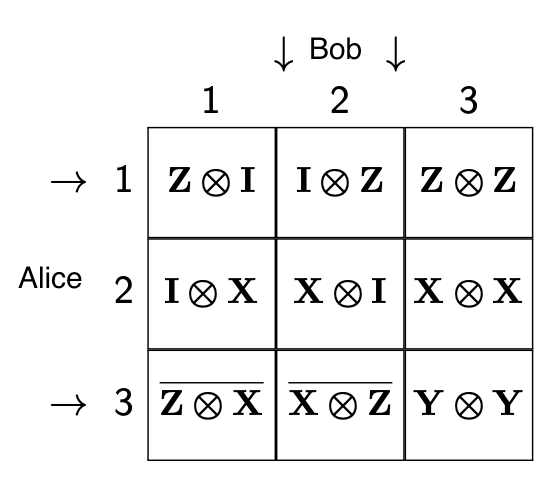
\includegraphics[scale=0.6]{mp.png}\end{minipage} &
\raisebox{1.2in}{\begin{minipage}[t]{3in}\raggedright Alice, having traveled to Israel, decides to compute her squares' results \textbf{right to left}, while Bob, still in St.~Louis (he turned down a trip to Australia), reports his results top to bottom, as usual.\end{minipage}}
\end{tabular}

\begin{enumerate}

\item\Points{2} With this change to Mermin--Peres, answer the following questions, assuming error-free quantum computations:

\begin{itemize}
    \item For any of her three rows, Alice \emph{always} reports values whose products are $+1$ as required.~\TF{}
    \item Alice and Bob \emph{always} agree on a value in their common square.~\TF{}

\end{itemize}
\item\Points{4} Below, explain your answers to part~(a), by providing an example that makes a statement false, or by explaining why the statement is true.
    \LeaveSpace{1in}

\item\Points{4} Alice and Bob are assigned row~2 and column~2, respectively. Suppose Alice happens to measure first, measuring $\ket{++}$ for her (first and rightmost) $\X{}\otimes\X{}$ square.

Fill in the blanks below showing \emph{all possible values} that could be reported by Alice and Bob, as they examine their squares in the order below, following Alice's initial measurement of the rightmost square in row 2.

\medskip

\begin{tabular}{cc}
\begin{minipage}{3in}
Alice row 2
\begin{itemize}
    \item Right square \Blank[4em]{}
    \item Center square \Blank[4em]{}
    \item Left square \Blank[4em]{}
\end{itemize}
\end{minipage}
&
\begin{minipage}{3in}
Bob column 2
\begin{itemize}
    \item Top square \Blank[4em]{}
    \item Middle square \Blank[4em]{}
    \item Bottom square \Blank[4em]{}
\end{itemize}
\end{minipage}
\end{tabular}
\end{enumerate}

\clearpage\item\Points{15}

\begin{enumerate}
Consider a qubit in state
\( \ket{\psi} = \frac{1}{\sqrt{2}}\SQB{i}{1}\)

\item\Points{3} We wish to measure this state in the \X{} basis, but alas we can only perform measurements on quantum computers in the computational (\Z) basis.  Put the following operations in the correct order (1, 2, 3) by writing the appropriate numerals in the blanks provided:
\begin{itemize}
    \item \Blank{} We map the \X{} basis to the \Z{} basis using an \H{} gate.

    \item \Blank{} We map the \Z{} basis to the \X{} basis using an \H{} gate.
        \item \Blank{} We measure in the computational basis.
\end{itemize}
\item\Points{8} For a nice change, suppose we want to measure state $\ket{\psi}$ in the Y{} basis. Recall that the \Y{} basis is spanned by 
\[ \ket{+y} = \frac{1}{\sqrt{2}}\SQB{1}{i} \mbox{ and } \ket{-y} = \frac{1}{\sqrt{2}}\SQB{1}{-i} \]
in the same way \Z{} is spanned by \ket{0} and \ket{1}, and \X{} is spanned by \ket{+} and \ket{-}.

Here we want to measure in the \Y{} basis.

The matrix that transform state from the \Z{} basis to \Y{}, mapping \ket{0} to \ket{+y} and \ket{1} to \ket{-y} is (use the blank to the left of the matrix for a common fraction, if you like):
\[
\raisebox{-1em}{\Blank[2.5em]{}}\begin{pmatrix*}[r]
  \Blank[2em]{} & \Blank[2em]{} \\
  \Blank[2em]{} & \Blank[2em]{} 
\end{pmatrix*}
\]
and its inverse is (be sure to conjugate as needed):
\[
\raisebox{-1em}{\Blank[2.5em]{}}\begin{pmatrix*}[r]
  \Blank[2em]{} & \Blank[2em]{} \\
  \Blank[2em]{} & \Blank[2em]{} 
\end{pmatrix*}
\]
\item\Points{4} Measuring \( \ket{\psi} = \frac{1}{\sqrt{2}}\SQB{i}{1}\) in the \Y{} basis yields \Blank{}.
\begin{quote}
    Hint:  You can find this answer without performing any matrix multiplication.
\end{quote}

\end{enumerate}
\clearpage\item\Points{10}

\mbox{}\vskip -5em\mbox{}\begin{center}
\begin{minipage}[t]{2.8in}
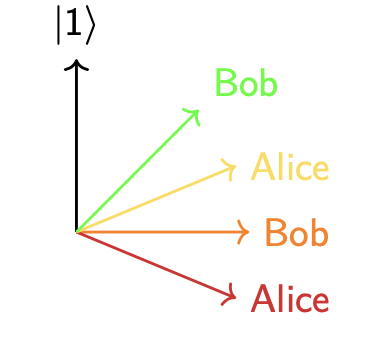
\includegraphics[scale=0.65]{chsh.png}\end{minipage}\end{center}


\begin{itemize}
\item Recall that in the CHSH solution, the angle between adjacent rays in the picture above is $\pi/8$, so that the probability of agreement where it should happen is approximately~$85\%$.
\item Suppose the angle between each adjacent pair of rays is changed to $\pi/16$, so that when they should agree, their probability of agreement is now
\[ \cos^{2}(\pi/16) \approx 96\% \]
and some other computations:
\begin{align*}
    \cos^{2}(2\pi/16) \approx 85\% \\
    \cos^{2}(3\pi/16) \approx 70\% \\
    \cos^{2}(4\pi/16) \approx 50\%
\end{align*}
\end{itemize}

All other aspects of the game are unchanged:  
\begin{itemize}
    \item Alice and Bob are provided colors that are chosen randomly and uniformly.
    \item The metric for \emph{success} of the game is the \emph{average} rate at which Alice and Bob agree when they should, and disagree when they should, over all 4 possible combinations of colors they can be provided. 
    \item In the game's solution using the above diagram, as taught, the \emph{success} metric is approximately~85\%.
\end{itemize}
Answer the following:
\begin{itemize}
    \item\Points{1} This change improves the \emph{success} of the game.~\TF{}.
    \item\Points{5} What is the approximate success metric of the game with this change? (provide a numeric answer, such as ``85'' for ``85\%'') \Blank{}\%
    \item\Points{3} Show the math supporting your answers below:
    \LeaveSpace{2in}
\end{itemize}

\clearpage\item\Points{10}
During an iteration of Grover, and after the first step (reflection) but before the second step (diffusion), we have obtained the following state:
\[
\ket{\psi_{f}} = \begin{pmatrix*}[r]
   0.25 \\
   0.25 \\
   0.25 \\
   0.25 \\
   0.25 \\
   -0.25 \\
   0.25 \\
   0.25 \\
     0.25 \\
   0.25 \\
   0.25 \\
   0.25 \\
     0.25 \\
   0.25 \\
   0.25 \\
   0.25 
\end{pmatrix*}
\]

\begin{quote}\bf
Important:  The column's first index is 0 and its last index is 15.\end{quote}

\begin{enumerate}
    \item This is an instance of Grover for a function, where the input values are \Blank{} bits wide.
    \item From $\ket{\psi_{f}}$ shown above, what is the secret \ket{w} (the input value that Grover is trying to find)?~\Blank{}
    \item This is the first step of the \Blank{} iteration of the algorithm.
    \item When we complete this iteration by performing diffusion, the amplitude on \ket{w} will be approximately \Blank{}, because it increases each iteration on a problem of this size by approximately~\Blank{}.
    
    
\end{enumerate}

\clearpage\item\Points{5} You are at a party where everybody is talking about quantum computing.  You overhear somebody pontificating about Bernstein--Vazirani problems of $n$ bits, namely functions of the form
\( f(x) = x \cdot s \),
where $x$ and $s$ are each $n$ bits wide.  

After one too many Negronis, the person claims that \emph{all} values of $s$ lead to balanced functions for the Deutsch--Jozsa problem.

Not so fast, you say.  That is almost true.  Yes, in terms of $n$ there are $\Theta\left(\mbox{\vrule width 0pt height 2em depth 0pt\raisebox{-1.5em}{\Blank[2.2em]}}\right)$ such functions, but for one value of $s$, namely $s=\Blank{}$, $f(x)=x\cdot s$ is not a balanced function; it is, in fact, constant.

OK the pontificator concedes, you are right\footnote{At least, Cytron hopes you got this right; sadly, he was not invited to this party}, but for all other values of $s$, the Bernstein--Vazirani functions provide \emph{all} oracles that are balanced to Deutsch--Jozsa: there are no others.

Thundering superpositions, you exclaim, that cannot be the case.  And you continue by providing a single-qubit example\footnote{the crowd gasping in awe at the elegance and simplicity of your counterexample} of a function that is balanced, but not of the form $f(x)=x\cdot s$ for any $s$:
\begin{align*}
    f(0) &= \Blank{} \\
    f(1) &= \Blank{}
\end{align*}
You then draw the oracle for this function on a conveniently provided napkin (just draw gates as needed over what you see below):

\begin{center}
\adjustbox{valign=t,scale=2.0}{\begin{quantikz}
\lstick{$x$} &  \qw & \qw & \qw & \qw & \rstick{$x$}\\[1.5em]
\lstick{$y$} &  \qw & \qw & \qw & \qw & \rstick{$y\oplus f(x)$}\\
\end{quantikz}}\end{center}

Be certain your oracle provides both of the outputs as required and shown above.






\clearpage\item\Points{5} Using Shor's algorithm, let's try to factor the number~35 using the following table of values for
\[ 2^{i} \mbox{ mod 35} \]
\begin{center}
\begin{tabular}{c|c}
  $i$ & $2^{i}\mbox{ mod 35}$ \\\hline
  0 & 1 \\
  1 &  2 \\
2 &  4 \\
3 &  8 \\
4 &  16 \\
5 &  32 \\
6 &  29 \\
7 &  23 \\
8 & 11 \\
9 &  22 \\
10 &  9 \\
11 & 18 \\
12 &  1
\end{tabular}
\end{center}
\begin{itemize}
    \item What is the period of this function?\Blank{}
    \item $2$ is a suitable base for using Shor's algorithm to factor~35 because the period of $2^{i}\mbox{ mod 35}$ is even~\TF{}.
    \item To find the factors of 35 we would perform the following computations:
    
     GCD(\Blank[3em]{},35) = \Blank[3em]{}
        
        and 
        
        GCD(\Blank[3em]{},35) = \Blank[3em]{}
    
\end{itemize}


\end{enumerate}

\end{assignment}
\Bpage{}

\end{document}
